\subsection{Datasets}

\subsubsection{T-Less 17}

The T-Less dataset was created by Hoda{\v{n}} et al.\cite{hodan_wacv2017} and serves as a benchmark for object detection and 6 \acrshort{DoF} pose estimation.
It provides range data for the Kinectv2 and PrimeSense Carmine 1.09 depth sensors.
Each sensor is modelled as pinhole camera and the calibration is provided by the dataset (see Table~\ref{tab:intrinsic_tless}).
{\renewcommand{\arraystretch}{1.2}%
\setlength{\tabcolsep}{1em}%
\begin{table}
    \begin{tabular}[H]{rrr}
    \toprule
    \textbf{Parameter} & \textbf{Kinectv2} & \textbf{PrimeSense} \\
    \midrule
    Principle & \acrshort{ToF} & structured light \\
    Resolution & \multicolumn{2}{c}{$400 \times 400px$} \\
    $(f_x, f_y)$ & $(1076.74, 1075.18)$ & $(1075.65, 1073.90)$ \\
    $(c_x, c_y)$ & $(213.98, 148.59)$ & $(225.07, 167.72)$ \\
    \bottomrule
    \end{tabular}
    \caption{Intrinsic parameters for the Kinectv2 and PrimeSense sensor, provided by the T-Less dataset.}\label{tab:intrinsic_tless}
\end{table}}

\begin{figure}[H]
    %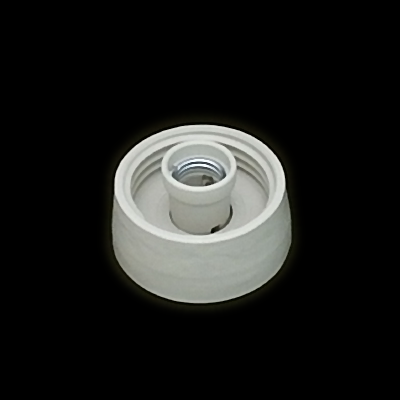
\includegraphics[width=0.5\linewidth]{chapter05/img/tless/color_0300.png}%
    
\includegraphics[width=0.25\linewidth]{chapter05/img/tless/kinect_bearing_0300.png}%
    
\includegraphics[width=0.25\linewidth]{chapter05/img/tless/kinect_flexion_0300.png}%
    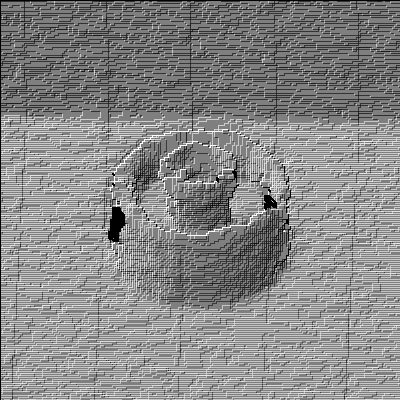
\includegraphics[width=0.25\linewidth]{chapter05/img/tless/primesense_bearing_0300.png}%
    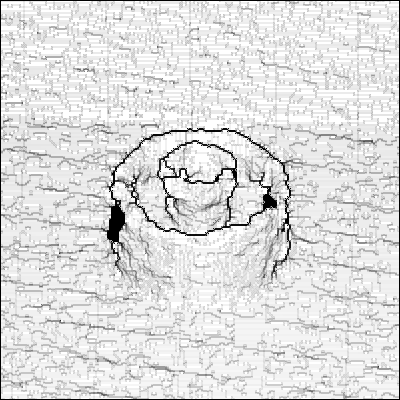
\includegraphics[width=0.25\linewidth]{chapter05/img/tless/primesense_flexion_0300.png}\\
\end{figure}

\subsubsection{Intel Realsense Static Scene}

{\renewcommand{\arraystretch}{1.2}%
\setlength{\tabcolsep}{1em}%
\begin{table}
    \begin{tabular}[H]{rc}
    \toprule
    \textbf{Parameter} & \textbf{Intel RealSense} \\
    \midrule
    Principle  & structured light \\
    Resolution & 400 $\times$ 400px \\
    $f_x$ & 1076.7406 \\
    $f_y$ & 1075.1783 \\
    $c_x$ &  213.9826 \\
    $c_y$ &  148.5918 \\
    \bottomrule
    \end{tabular}
    \caption{Intrinsic parameters used for the Intel RealSense depth sensor.}
\end{table}}

Depth Resolution not good enough.
Intel Realsense Sensor

\subsubsection{Synthetic Blender Scene}

The first synthetic dataset is a manually created scene in Blender\cite{blender}.
Both rotation and translation are done in isolation as well combined.
The scene consists of a sphere, a cylinder, a cube-like object with additional edges of different smootheness and a complex monkey head in a room (Figure~\ref{fig:blender_scene}).
The camera movement is rendered in an animation and the depth buffer of each frame is extracted as image.
From the rendering settings the camera matrix is calculated and its parameters provided in Table~\ref{tab:blender_intrinsic}.
\begin{figure}
\CenterFloatBoxes
\begin{floatrow}
    \btabbox{%
    \renewcommand{\arraystretch}{1.2}%
    \setlength{\tabcolsep}{1em}%
    \begin{tabular}{rc}
    \toprule
    \textbf{Parameter} & \textbf{Blender Camera} \\
    \midrule
    Principle  & Rendering \\
    Resolution & 1080 $\times$ 1080px \\
    $f_x$, $f_y$ & 2220.0, 2220.0 \\
    $c_x$, $c_y$ &  540.0, 540.0 \\
    \bottomrule
    \end{tabular}}
    {\caption{Blender camera intrinsic}\label{tab:blender_intrinsic}}%
    \ffigbox{
    
\includegraphics[width=0.5\linewidth]{chapter05/img/blender/blender_render01.png}%
    
\includegraphics[width=0.5\linewidth]{chapter05/img/blender/depth_image_scene0005.png}%
    }
    {\caption{One frame as normal render and depth image.}\label{fig:blender_scene}}
\end{floatrow}
\end{figure}
The total animation consists of 211 images and no noise is applied to the depth image.

\subsubsection{Lehrpfad Kinect}

Kinectv2-data from a robot drive in the Reiche Zeche.
It provides groundthruth data from a prior reconstruction after global optimization.
It contains a loop closure and different section of the mining environment, from man made concrete walls to raw stone walls.
The groundthruth poses do not match the scale of the depth sensor anymore, as global optimization adjusted the translation too much.
The rotation is proper, each pose is adjusted with ICP that uses the provided pose as initial guess.

% \subsubsection{Office Kinect}

\subsubsection{Laserscans of Reiche Zeche - Wilhelm Stehender Süd}

LIDAR based high resolution scans that are used in the context of mine surveying.
Those scans are not made for robotic or computer vision purposes.
This is the reason, why they have little overlap between each scan.
Special reflectors are used as landmarks to register the point clouds to each other.
Only a subset of the scans is used in this evaluation, to demonstrate the functionality and generality of the approach.
Statistics of the distribution and response of the keypoints are provided.

\subsubsection{LIDAR and Pinhole Camera matching}

One advantage of the feature based approach is mixing highly different depth sensors with ease.
Examplaric scene with data from Kinectv2 sensor and the LIDAR that demonstrates, that matching between those two sensors is possible.
Demonstrate, that prior conversion from equirectangular to pinhole reduces the distortion and therefore change in appearance between different camera models.

% Lehrpfad Ziege ist auch im Wilhelm-Sued-Kinect Datensatz. Damit ist da Equi, +Laserscan Pinhole + Kinect vorhanden

\subsubsection{Synthetic City Scene}

City walkthrough that is used as odometry benchmark.

